%!TEX program = xelatex
\documentclass[11pt]{beamer}

\usepackage{amsfonts}
\usepackage{amsmath}
\usepackage{blindtext}
\usepackage{enumitem}
\usepackage{hyperref}
\usepackage{colortbl}
\usepackage{fancyvrb}
\usepackage{booktabs}

\hypersetup{pdfborder = {0 0 0}}

\usetheme{SaoPaulo}

\title{Welcome to CS \emph{101}!}
\subtitle{Introduction to Programming}
\author{CS101 Lecture \#1}
\date{2016-08-22}

\setcounter{showSlideNumbers}{1}

\begin{document}
  \setcounter{showProgressBar}{0}
  \setcounter{showSlideNumbers}{0}

%%%%%%%%%%%%%%%%%%%%%%%%%%%%%%%%%%%%%%%%%%%%%%%%%%%%%%%%%%%%%%%%%%%%%%%%%%%%%%%%
\frame{\titlepage}

%%%%%%%%%%%%%%%%%%%%%%%%%%%%%%%%%%%%%%%%%%%%%%%%%%%%%%%%%%%%%%%%%%%%%%%%%%%%%%%%
\setcounter{framenumber}{0}
\setcounter{showProgressBar}{1}
\setcounter{showSlideNumbers}{1}

%%%%%%%%%%%%%%%%%%%%%%%%%%%%%%%%%%%%%%%%%%%%%%%%%%%%%%%%%%%%%%%%%%%%%%%%%%%%%%%%
\section{Class Structure}

%%%%%%%%%%%%%%%%%%%%%%%%%%%%%%%%%%%%%%%%%%%%%%%%%%%%%%%%%%%%%%%%%%%%%%%%%%%%%%%%
\begin{frame}[plain,c]
  \frametitle{Class Website}
  \Enlarge

  \begin{center}
    \textcolor{CS101Base}{\Huge \texttt{go.illinois.edu/cs101}}
  \end{center}
\end{frame}

%%%%%%%%%%%%%%%%%%%%%%%%%%%%%%%%%%%%%%%%%%%%%%%%%%%%%%%%%%%%%%%%%%%%%%%%%%%%%%%%
\begin{frame}
  \frametitle{Grading}
  \begin{tabular}{*{27}{ll}}
    \toprule
    20\% & Homework \\
    25\% & Labs \\
    10\% & Lecture Participation \\
    20\% & Midterms \\
    25\% & Final Exam \\
    \bottomrule
  \end{tabular}
\end{frame}

%%%%%%%%%%%%%%%%%%%%%%%%%%%%%%%%%%%%%%%%%%%%%%%%%%%%%%%%%%%%%%%%%%%%%%%%%%%%%%%%
\begin{frame}
  \frametitle{Required Supplies}
  \Enlarge

  \begin{itemize}
    \myitem i>clicker \\ \textcolor{CS101GradBot}{\footnotesize\hspace{1em} Grades count starting Wed 08-31} \pause
    \myitem CodeLab account \\ \textcolor{CS101GradBot}{\footnotesize\hspace{1em} Instructions in \texttt{hw01}} \pause
    \myitem No textbook!
  \end{itemize}
\end{frame}

%%%%%%%%%%%%%%%%%%%%%%%%%%%%%%%%%%%%%%%%%%%%%%%%%%%%%%%%%%%%%%%%%%%%%%%%%%%%%%%%
\begin{frame}
  \frametitle{Homework Policies}
  \Enlarge

  \begin{itemize}
    \myitem No late homework submissions. \pause
    \myitem All machine-generated grades are final. \pause
    \myitem Late registrants should keep up with work. \\ \textcolor{CS101GradBot}{\footnotesize\hspace{1em} Corollary:  No extensions or exceptions for late registration.} \pause
    \myitem Get help at Piazza forum. \\ \textcolor{CS101GradBot}{\footnotesize\hspace{1em} Be civil to staff and peers. \\ All posts containing solutions should be marked as private.}
  \end{itemize}
\end{frame}

%%%%%%%%%%%%%%%%%%%%%%%%%%%%%%%%%%%%%%%%%%%%%%%%%%%%%%%%%%%%%%%%%%%%%%%%%%%%%%%%
\begin{frame}[plain,c]
  \frametitle{Class Website}
  \Enlarge

  \begin{center}
    \textcolor{CS101Base}{\Huge Lab \#1 begins today!}
  \end{center}
\end{frame}

%%%%%%%%%%%%%%%%%%%%%%%%%%%%%%%%%%%%%%%%%%%%%%%%%%%%%%%%%%%%%%%%%%%%%%%%%%%%%%%%
\section{Programming}

%%%%%%%%%%%%%%%%%%%%%%%%%%%%%%%%%%%%%%%%%%%%%%%%%%%%%%%%%%%%%%%%%%%%%%%%%%%%%%%%
\begin{frame}[fragile]
  \frametitle{Early mathematics}

  \begin{tabular}{cc}
  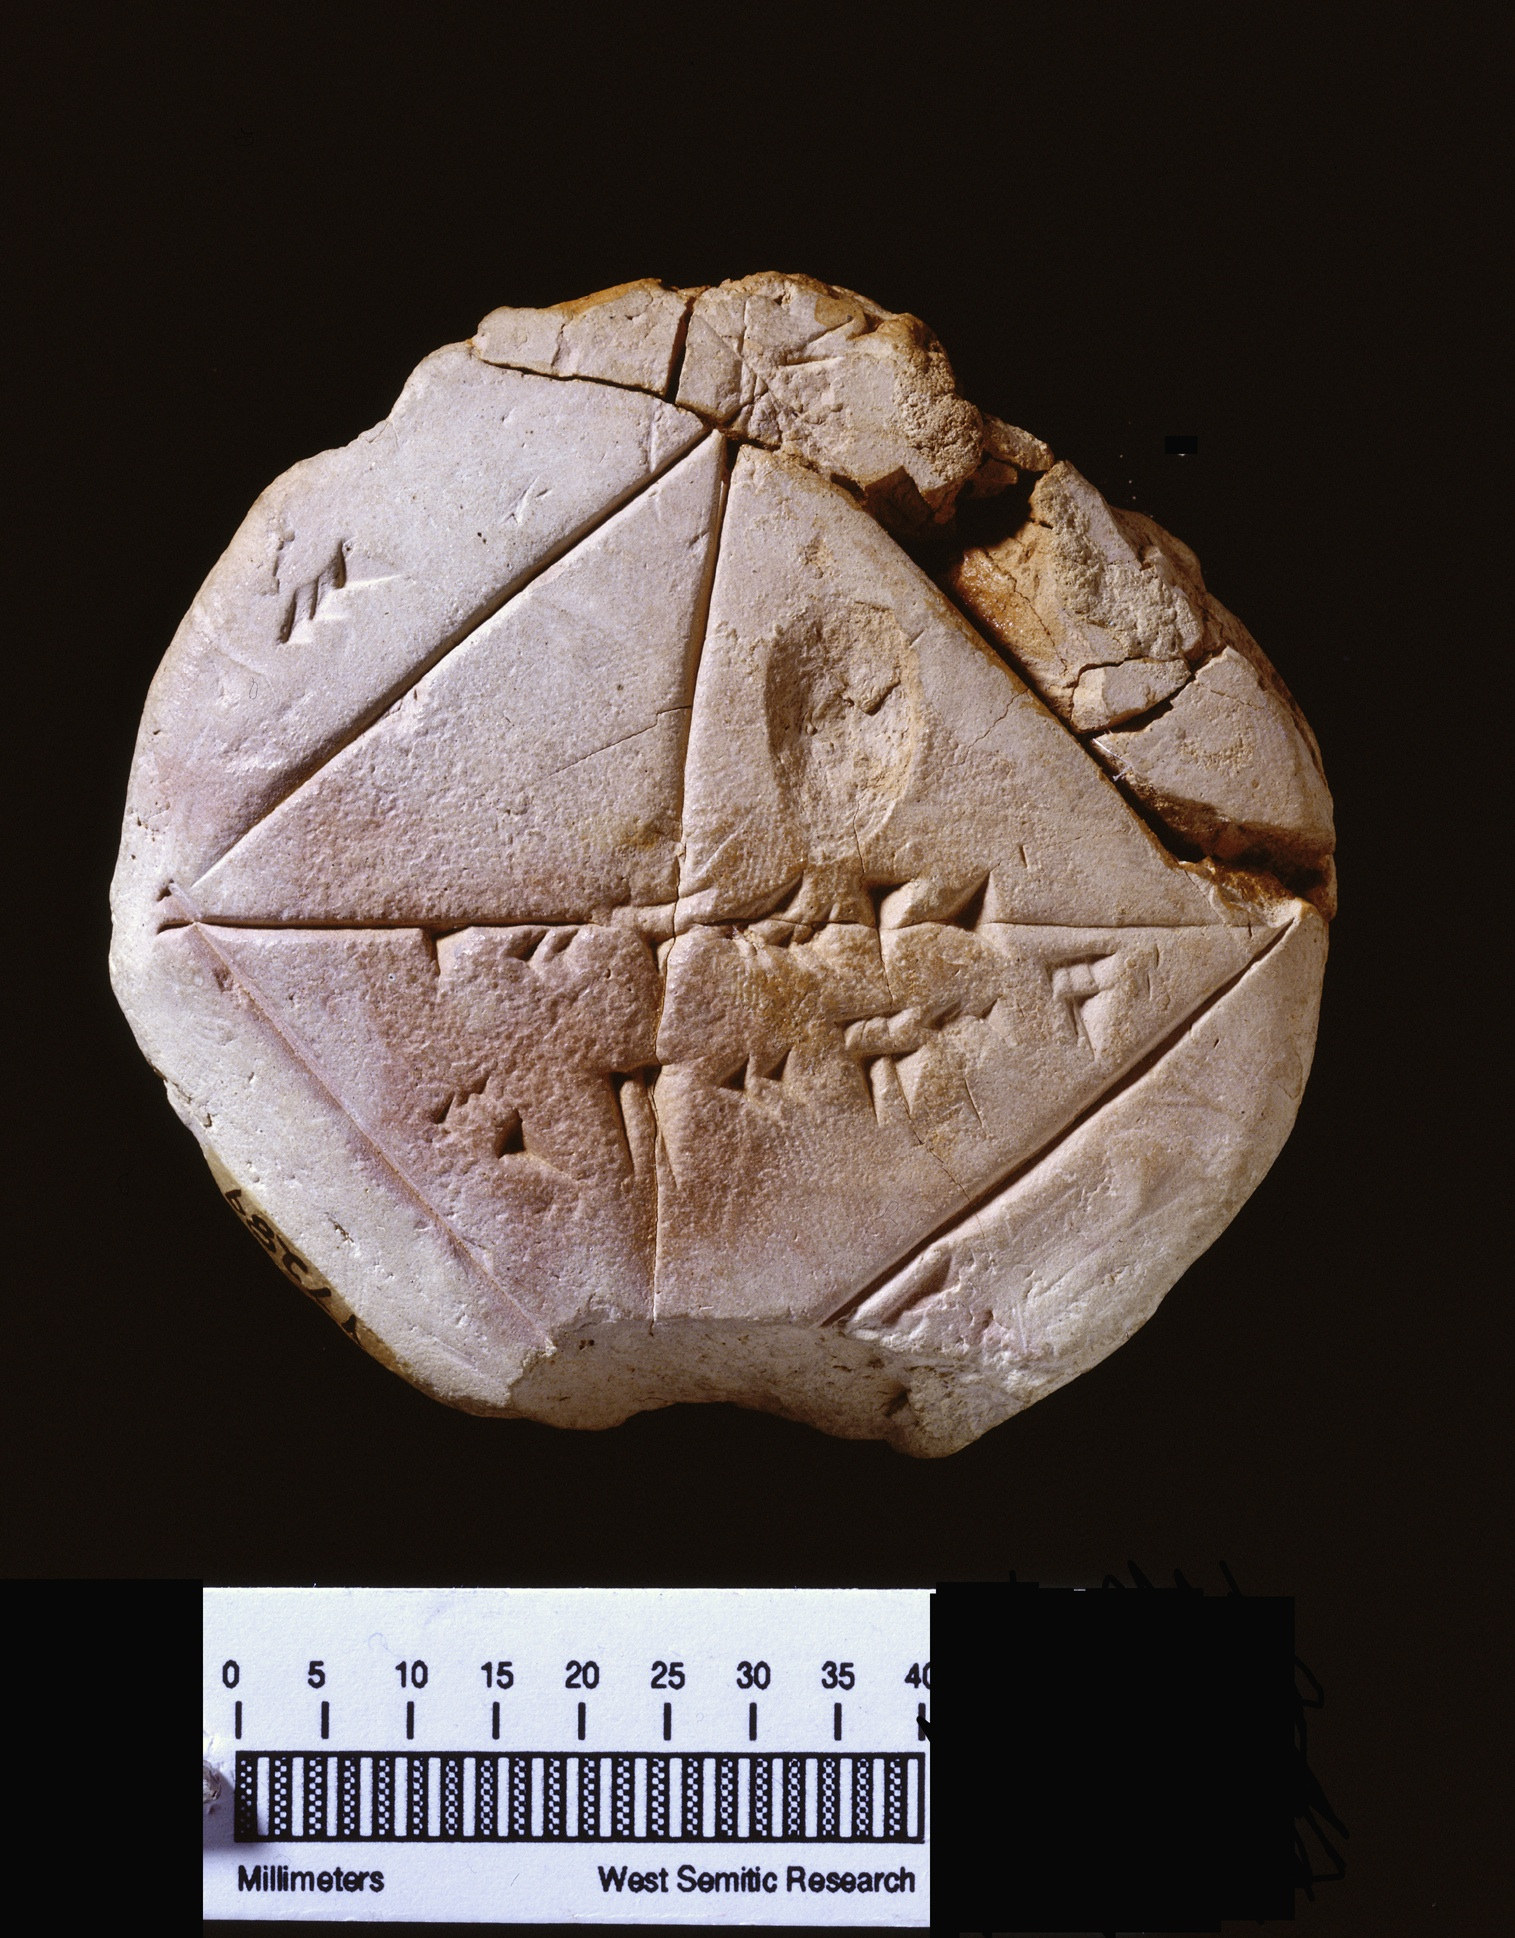
\includegraphics[height=0.75\textheight]{./img/ybc7289.jpg}
  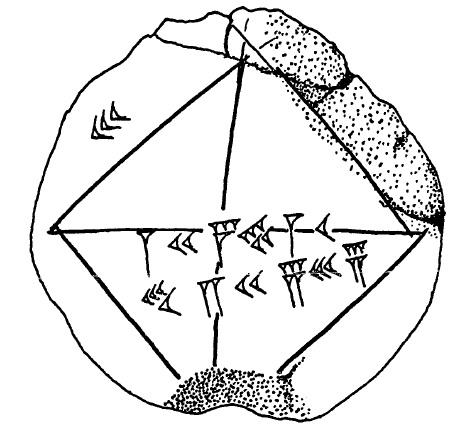
\includegraphics[height=0.375\textheight]{./img/ybc7289-schematic.jpg}
  \end{tabular}
\end{frame}

%%%%%%%%%%%%%%%%%%%%%%%%%%%%%%%%%%%%%%%%%%%%%%%%%%%%%%%%%%%%%%%%%%%%%%%%%%%%%%%%
\begin{frame}[fragile]
  \frametitle{Early mathematics}

  \begin{tabular}{cc}
  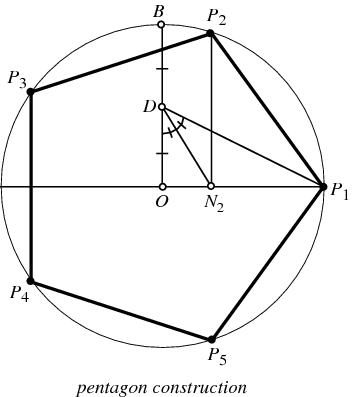
\includegraphics[height=0.75\textheight]{./img/pentagon.png}
  \end{tabular}
\end{frame}

%%%%%%%%%%%%%%%%%%%%%%%%%%%%%%%%%%%%%%%%%%%%%%%%%%%%%%%%%%%%%%%%%%%%%%%%%%%%%%%%
\begin{frame}[fragile]
  \frametitle{Early calculation}

  \includegraphics[height=0.25\textheight]{./img/abacus.jpg} \\
  \includegraphics[width=0.75\textwidth]{./img/pascal.jpg}
\end{frame}

%%%%%%%%%%%%%%%%%%%%%%%%%%%%%%%%%%%%%%%%%%%%%%%%%%%%%%%%%%%%%%%%%%%%%%%%%%%%%%%%
\begin{frame}[fragile]
  \frametitle{Early calculation}

  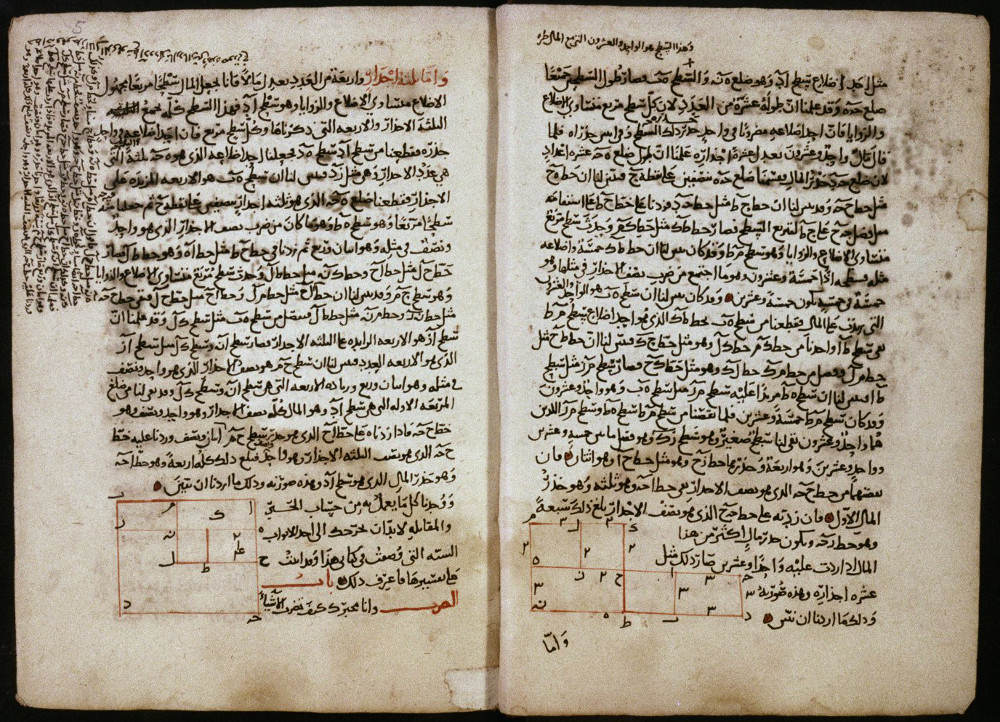
\includegraphics[height=0.75\textheight]{./img/al-khwarizmi.png}
\end{frame}

%%%%%%%%%%%%%%%%%%%%%%%%%%%%%%%%%%%%%%%%%%%%%%%%%%%%%%%%%%%%%%%%%%%%%%%%%%%%%%%%
\begin{frame}[fragile]
  \frametitle{Characteristica universalis}

  \begin{tabular}{cc}
  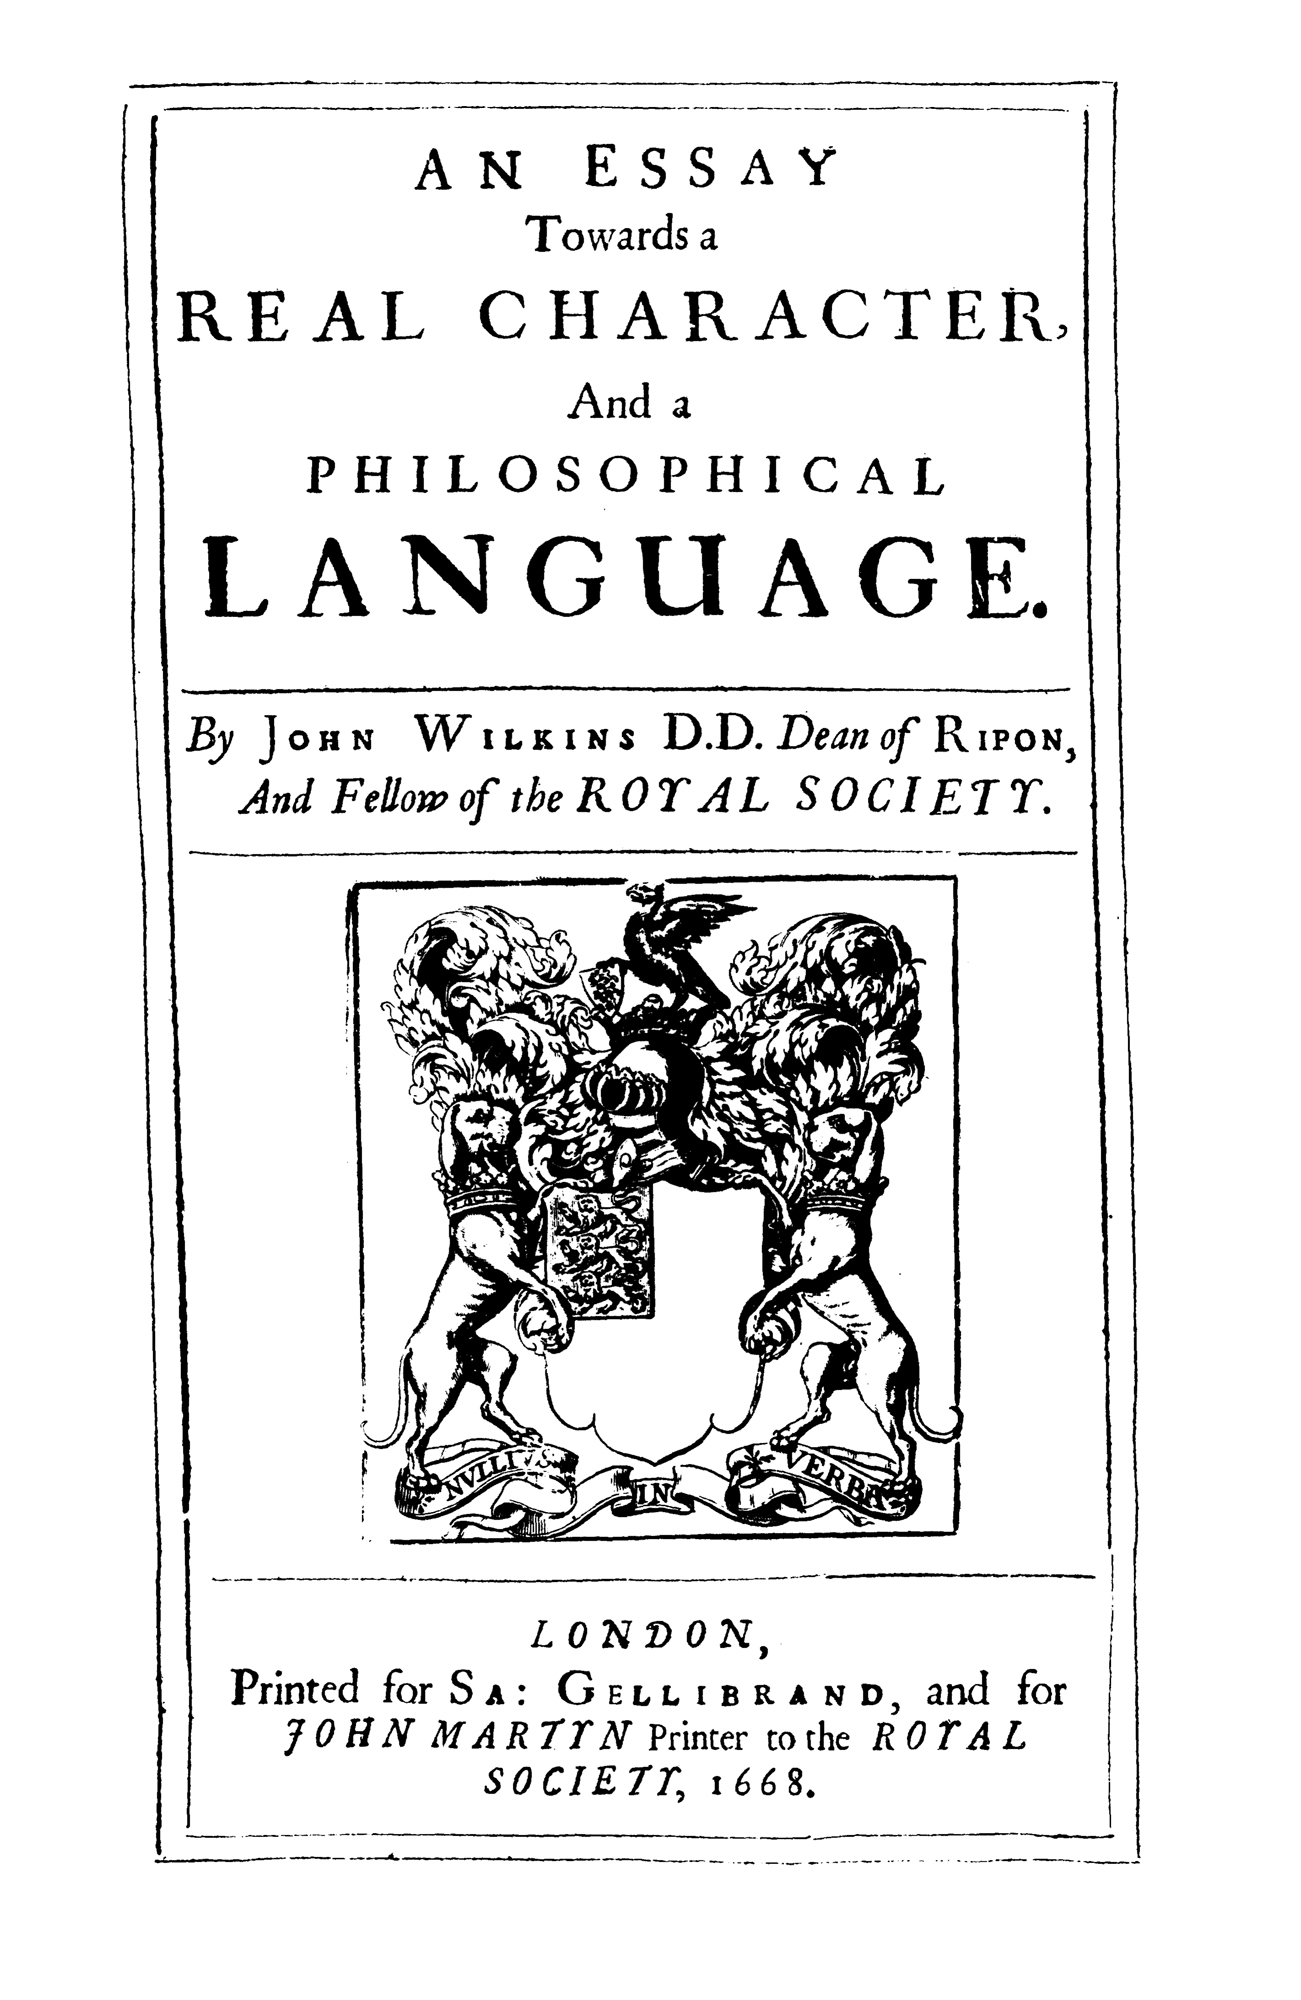
\includegraphics[height=0.75\textheight]{./img/wilkins.jpg}
  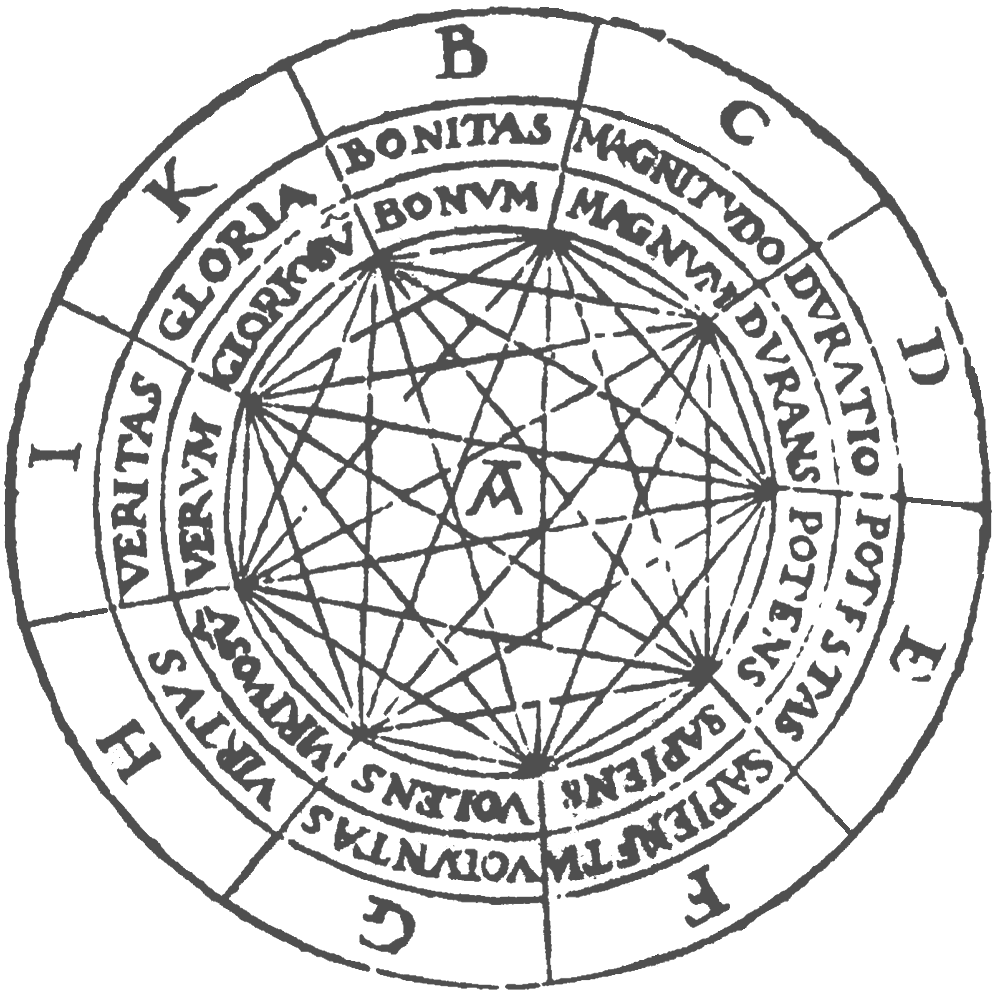
\includegraphics[width=0.5\textwidth]{./img/llull.png}
  \end{tabular}
\end{frame}

%%%%%%%%%%%%%%%%%%%%%%%%%%%%%%%%%%%%%%%%%%%%%%%%%%%%%%%%%%%%%%%%%%%%%%%%%%%%%%%%
\begin{frame}[fragile]
  \frametitle{Modern calculation}

  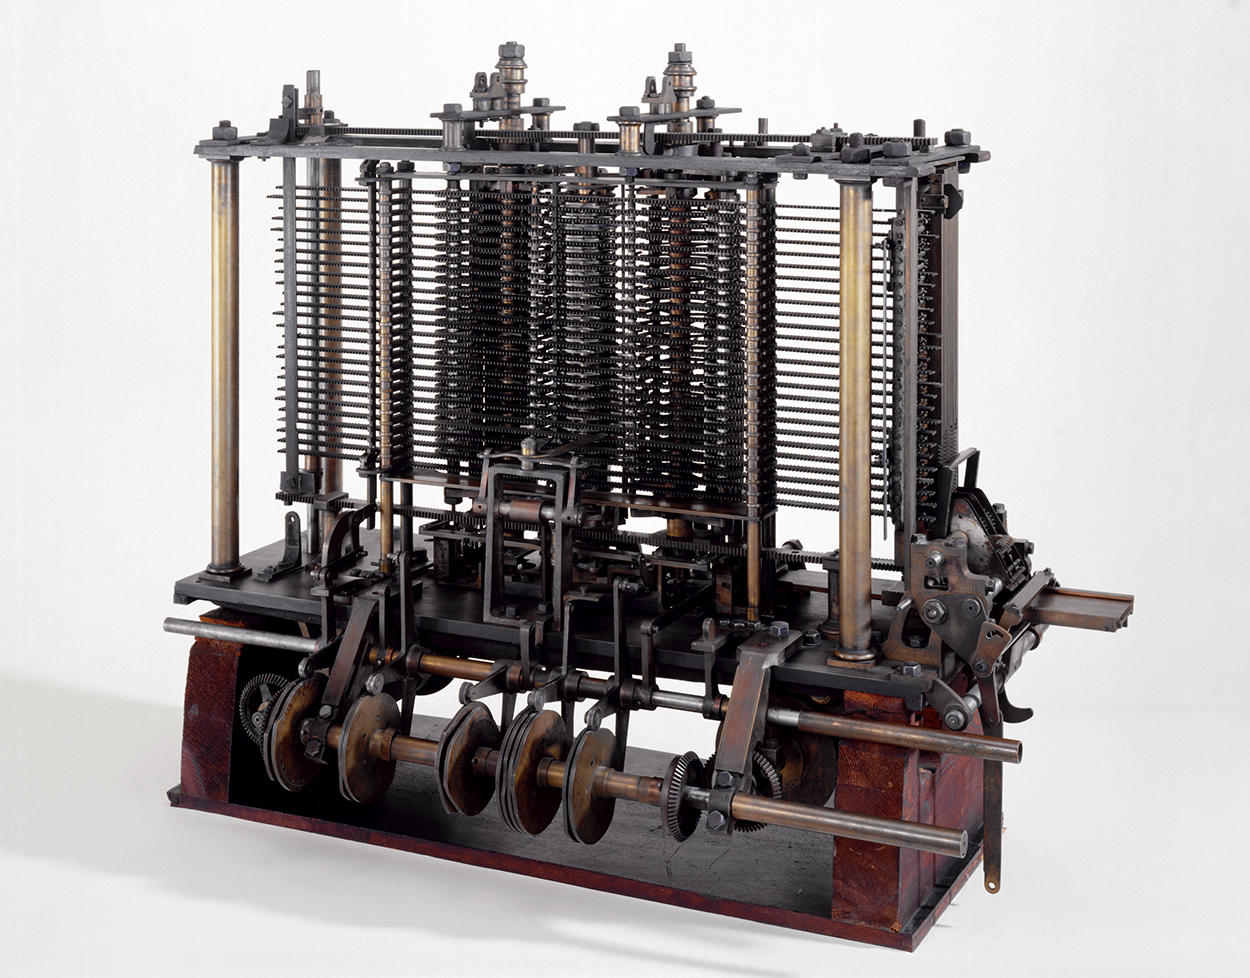
\includegraphics[height=0.75\textheight]{./img/babbage-1.jpg}
\end{frame}

%%%%%%%%%%%%%%%%%%%%%%%%%%%%%%%%%%%%%%%%%%%%%%%%%%%%%%%%%%%%%%%%%%%%%%%%%%%%%%%%
\begin{frame}[fragile]
  \frametitle{Modern calculation}

  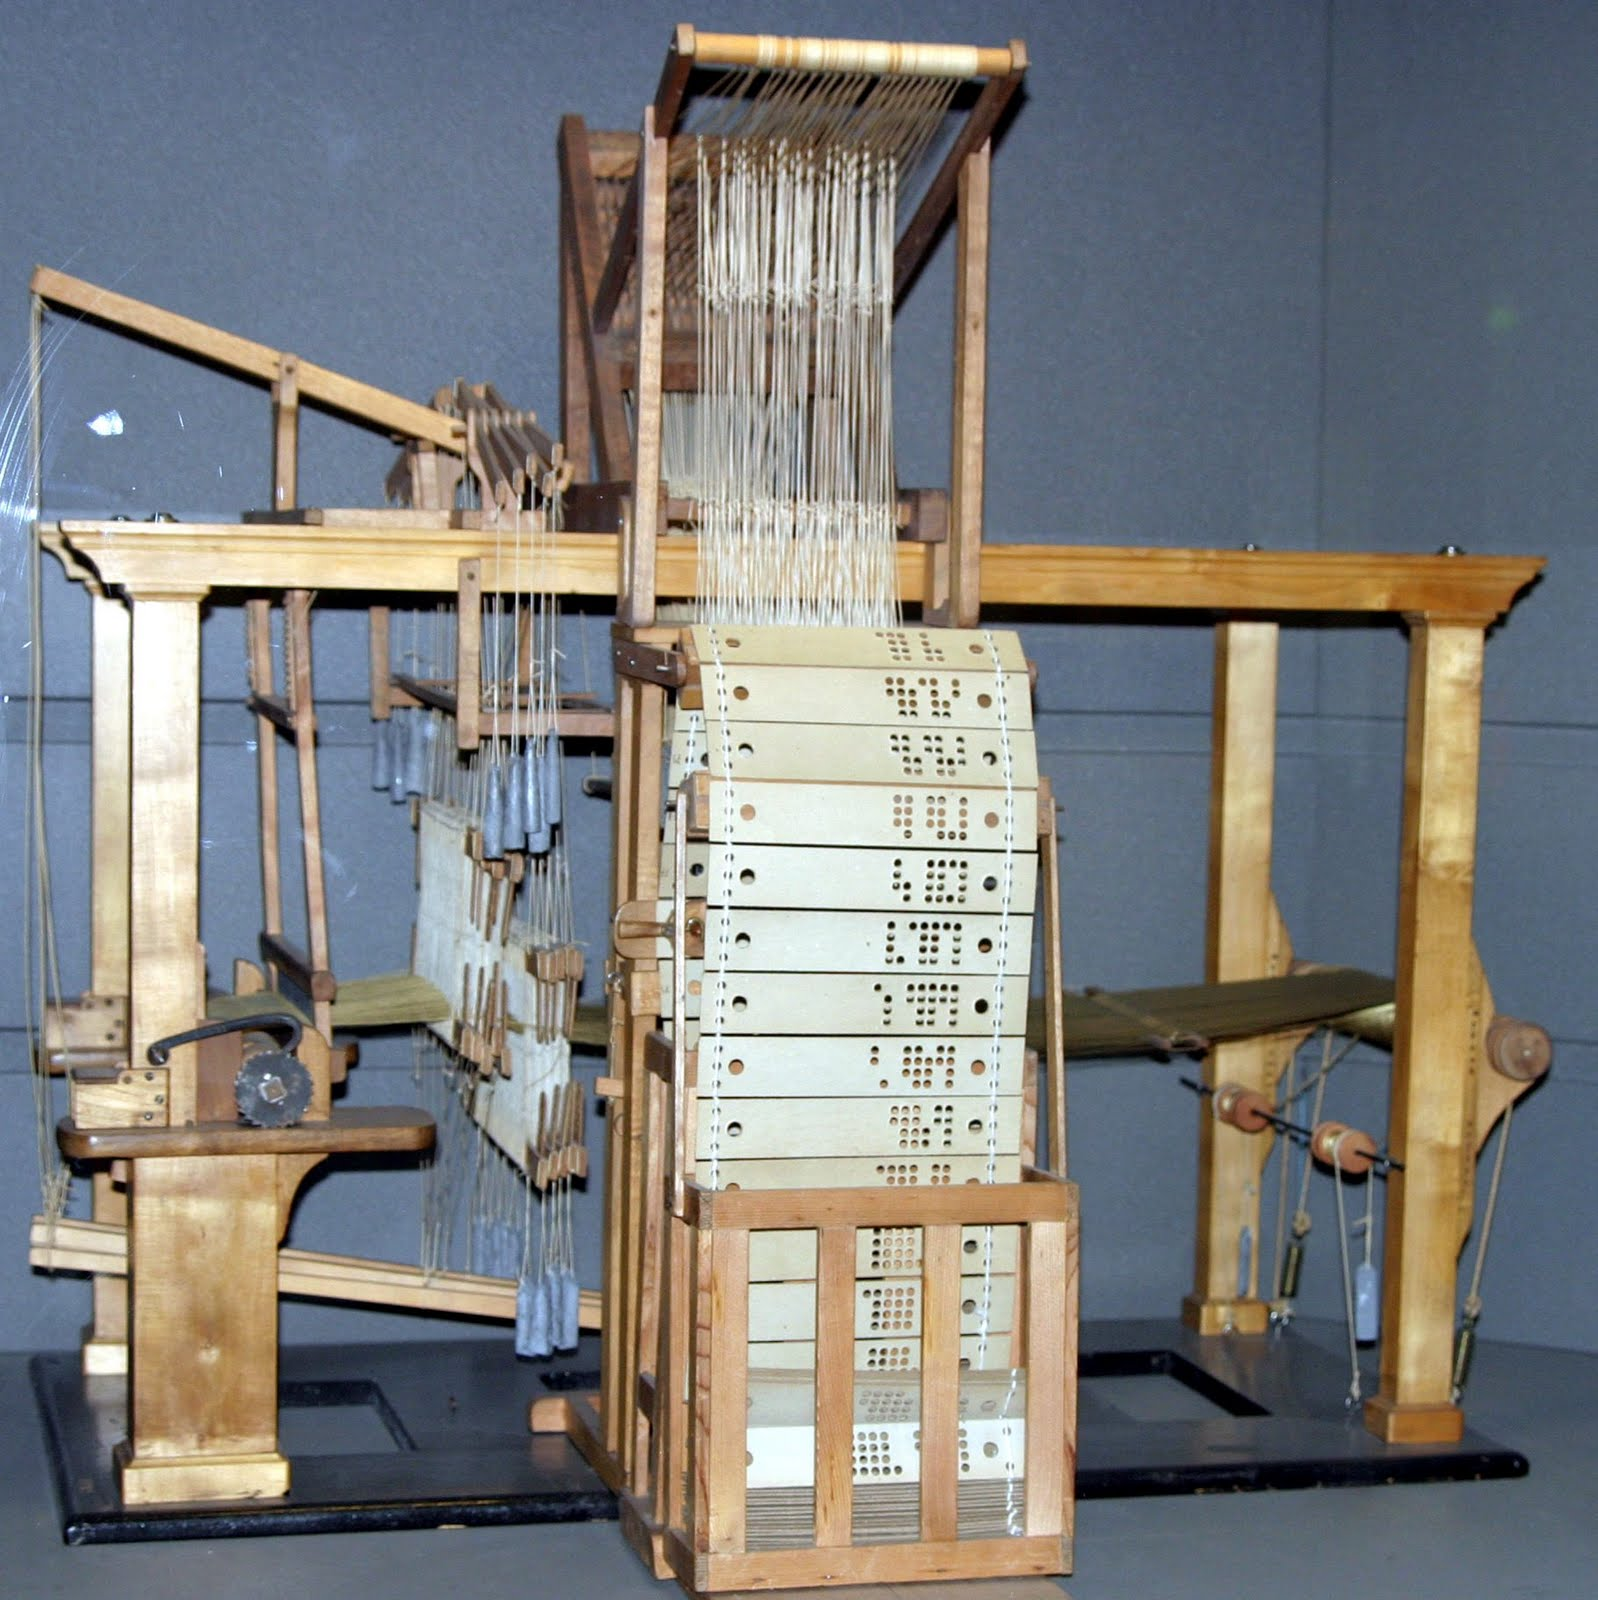
\includegraphics[height=0.75\textheight]{./img/jacquard.jpg}
\end{frame}

%%%%%%%%%%%%%%%%%%%%%%%%%%%%%%%%%%%%%%%%%%%%%%%%%%%%%%%%%%%%%%%%%%%%%%%%%%%%%%%%
\begin{frame}[fragile]
  \frametitle{Modern calculation}

  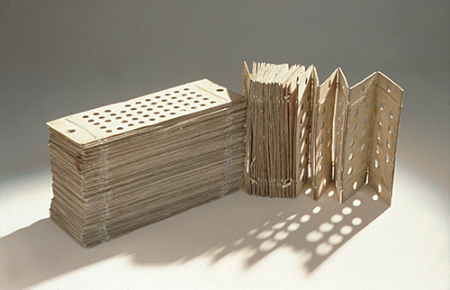
\includegraphics[height=0.75\textheight]{./img/babbage-2.png}
\end{frame}

%%%%%%%%%%%%%%%%%%%%%%%%%%%%%%%%%%%%%%%%%%%%%%%%%%%%%%%%%%%%%%%%%%%%%%%%%%%%%%%%
\begin{frame}[fragile]
  \frametitle{Modern calculation}

  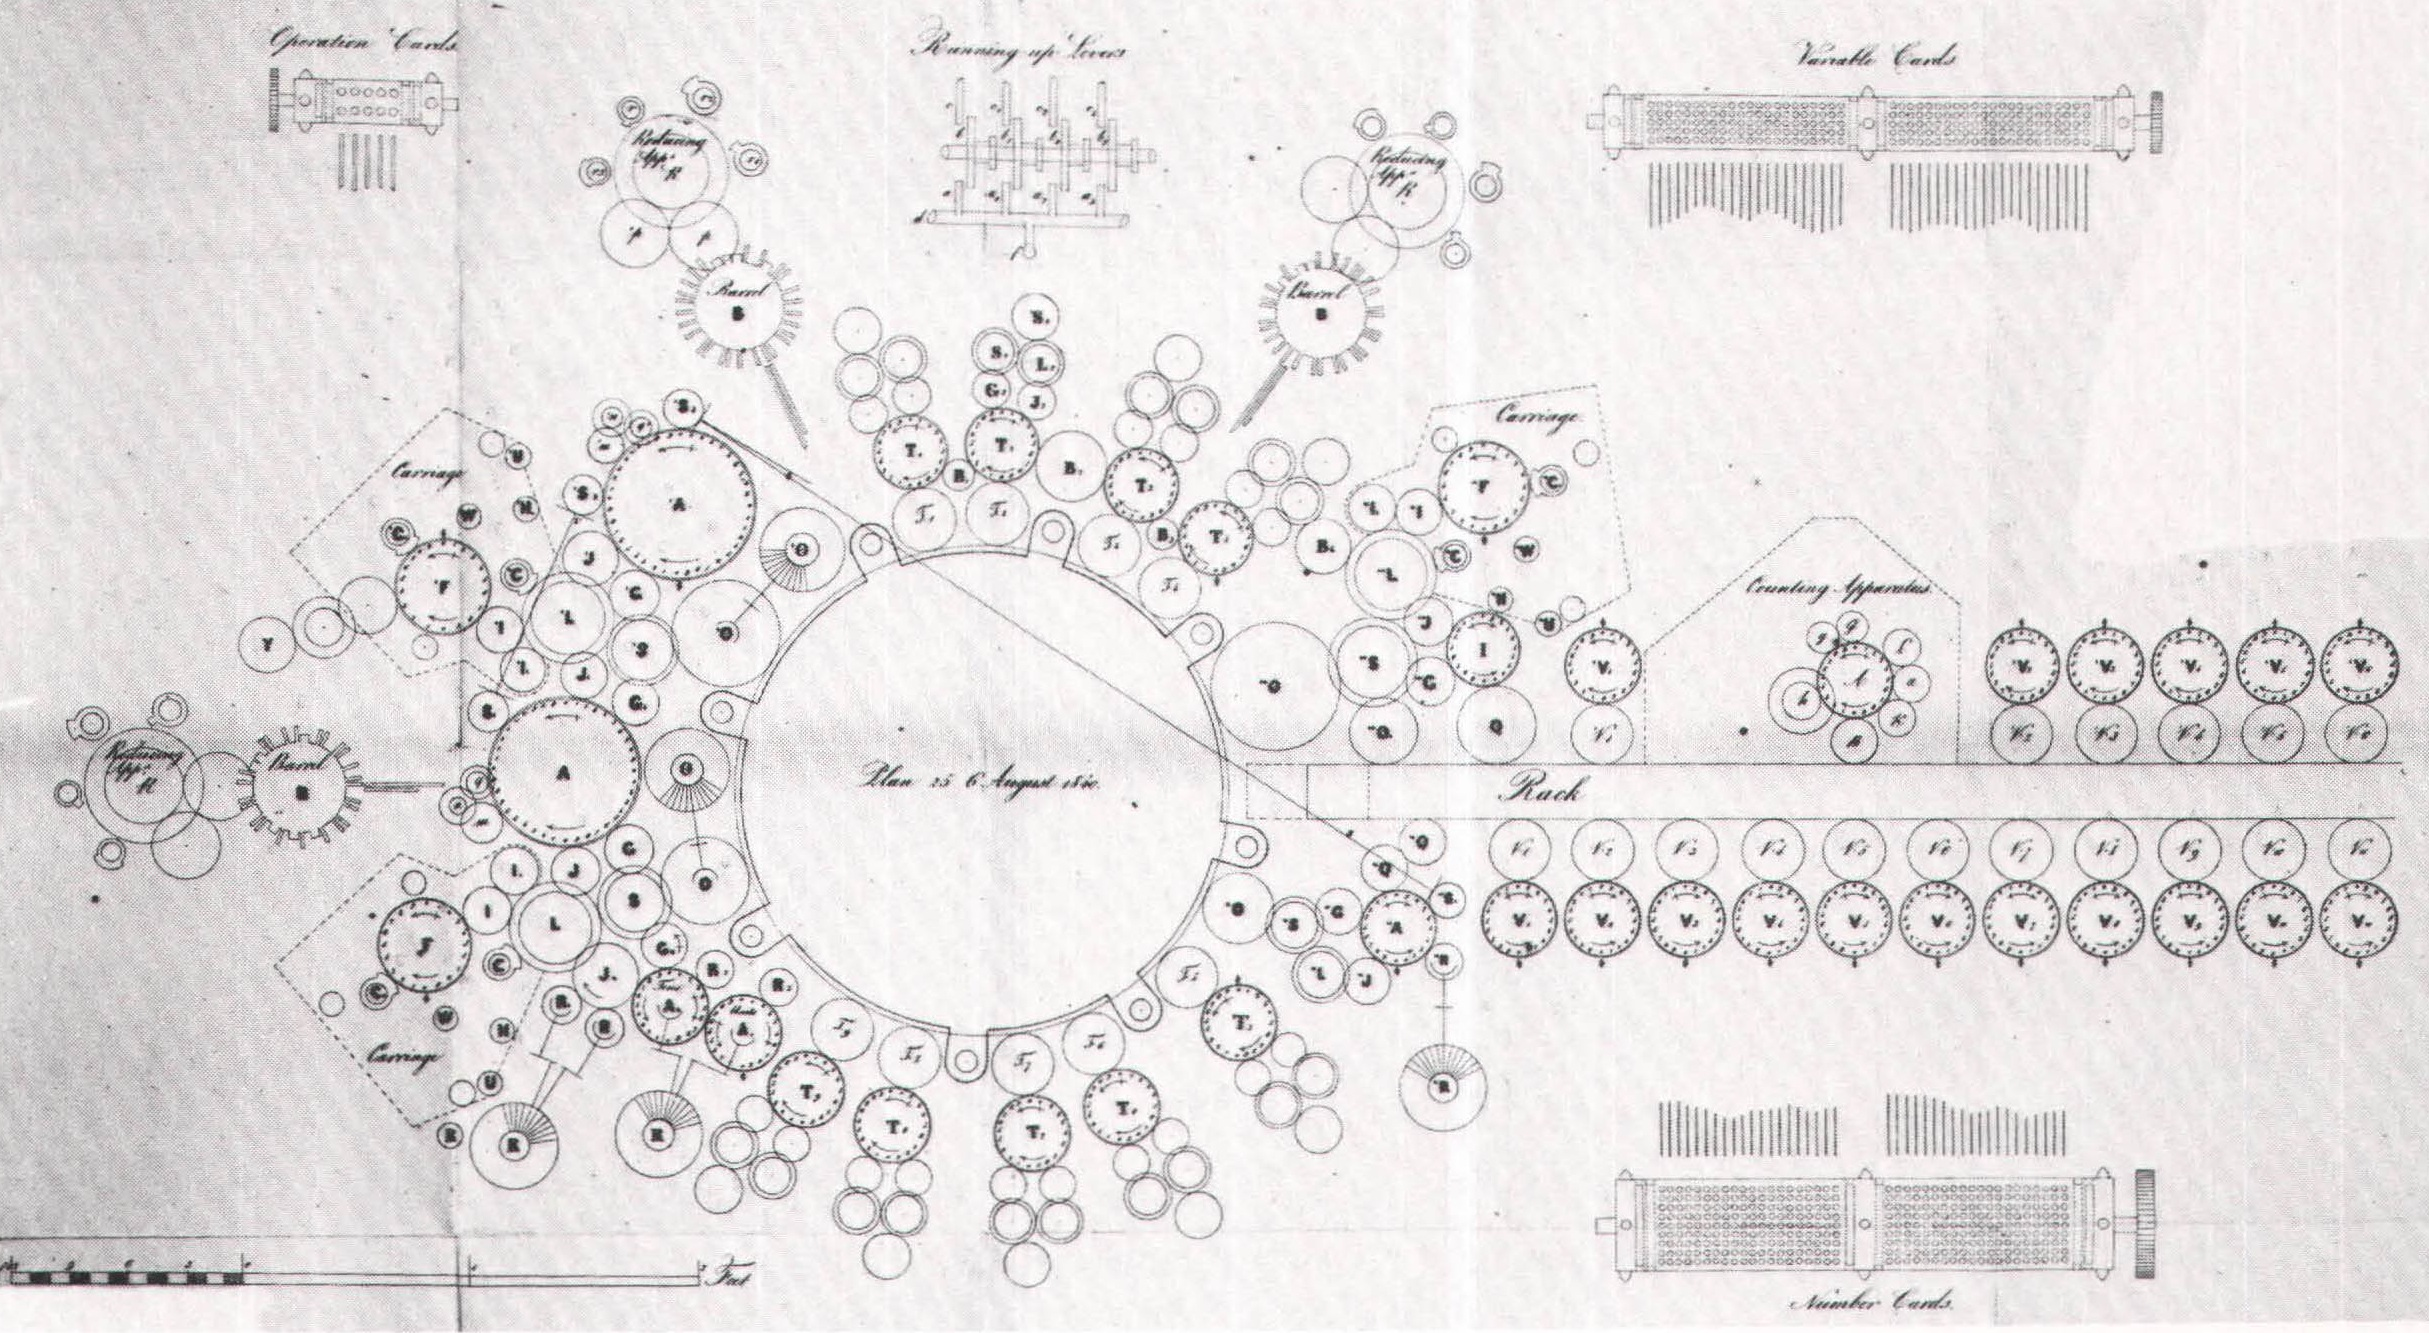
\includegraphics[height=0.75\textheight]{./img/babbage-3.jpg}
\end{frame}

%%%%%%%%%%%%%%%%%%%%%%%%%%%%%%%%%%%%%%%%%%%%%%%%%%%%%%%%%%%%%%%%%%%%%%%%%%%%%%%%
\begin{frame}[fragile]
  \frametitle{Modern calculation}

  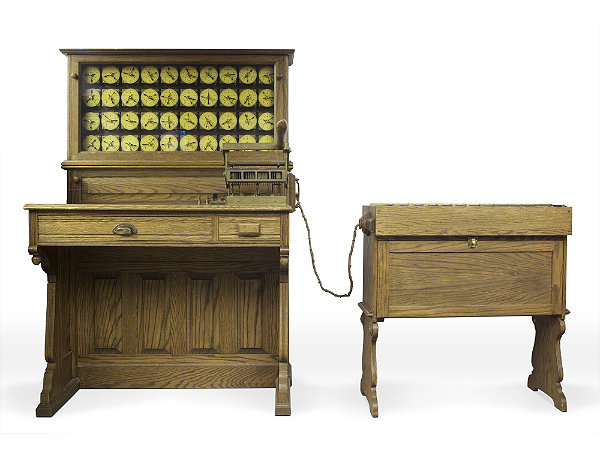
\includegraphics[height=0.75\textheight]{./img/ibm.jpg}
\end{frame}

%%%%%%%%%%%%%%%%%%%%%%%%%%%%%%%%%%%%%%%%%%%%%%%%%%%%%%%%%%%%%%%%%%%%%%%%%%%%%%%%
\begin{frame}[fragile]
  \frametitle{Modern calculation}

  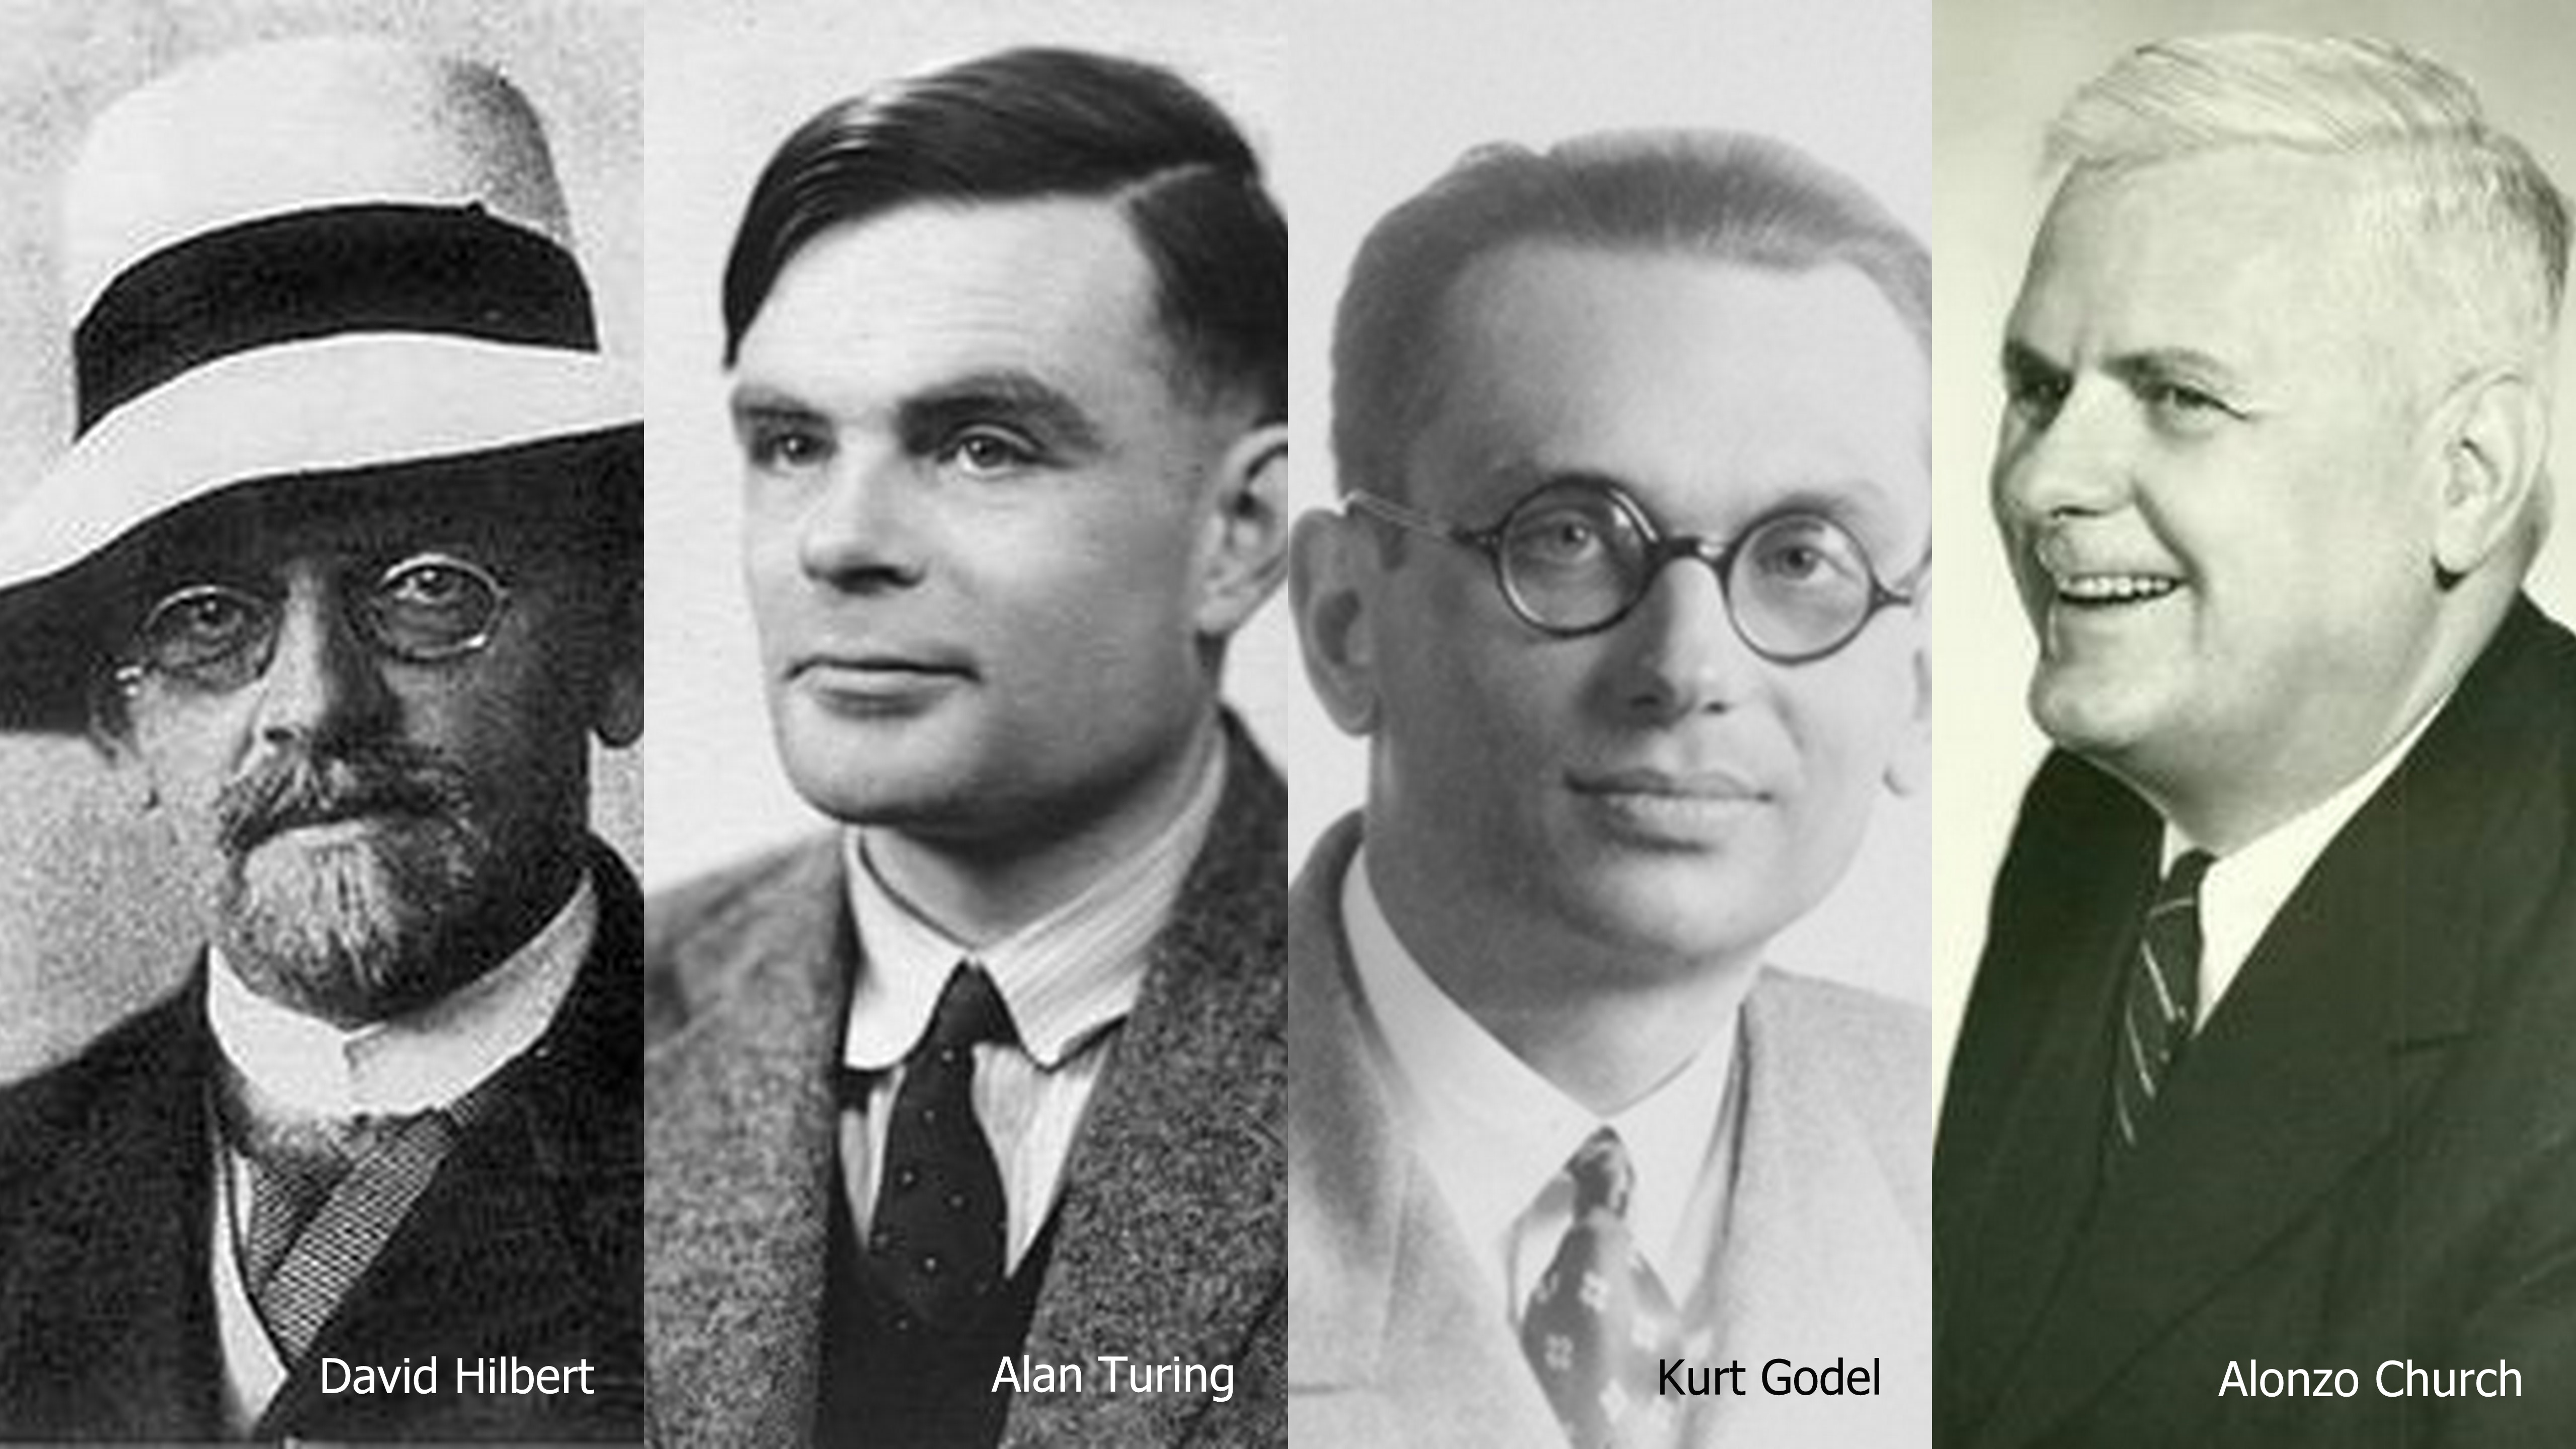
\includegraphics[width=\textwidth]{./img/turing-et-al.jpg}
\end{frame}

%%%%%%%%%%%%%%%%%%%%%%%%%%%%%%%%%%%%%%%%%%%%%%%%%%%%%%%%%%%%%%%%%%%%%%%%%%%%%%%%
\begin{frame}[fragile]
  \frametitle{Modern calculation}

  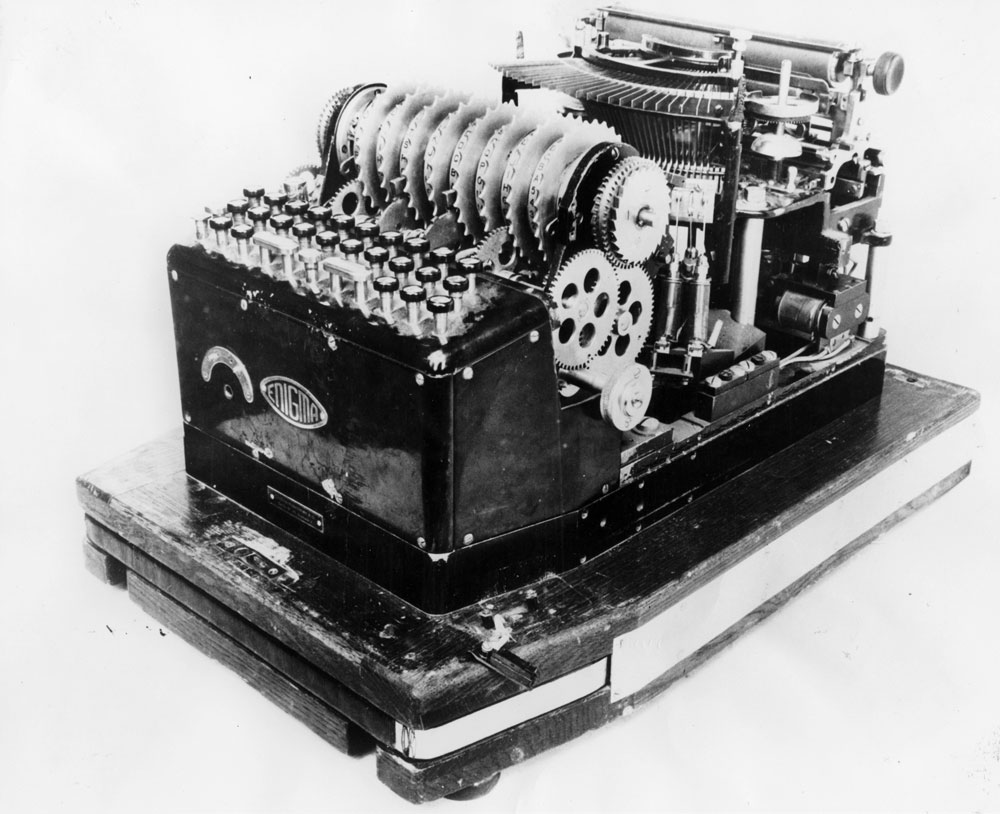
\includegraphics[height=0.75\textheight]{./img/enigma.jpg}
\end{frame}

%%%%%%%%%%%%%%%%%%%%%%%%%%%%%%%%%%%%%%%%%%%%%%%%%%%%%%%%%%%%%%%%%%%%%%%%%%%%%%%%
\begin{frame}[fragile]
  \frametitle{Modern calculation}

  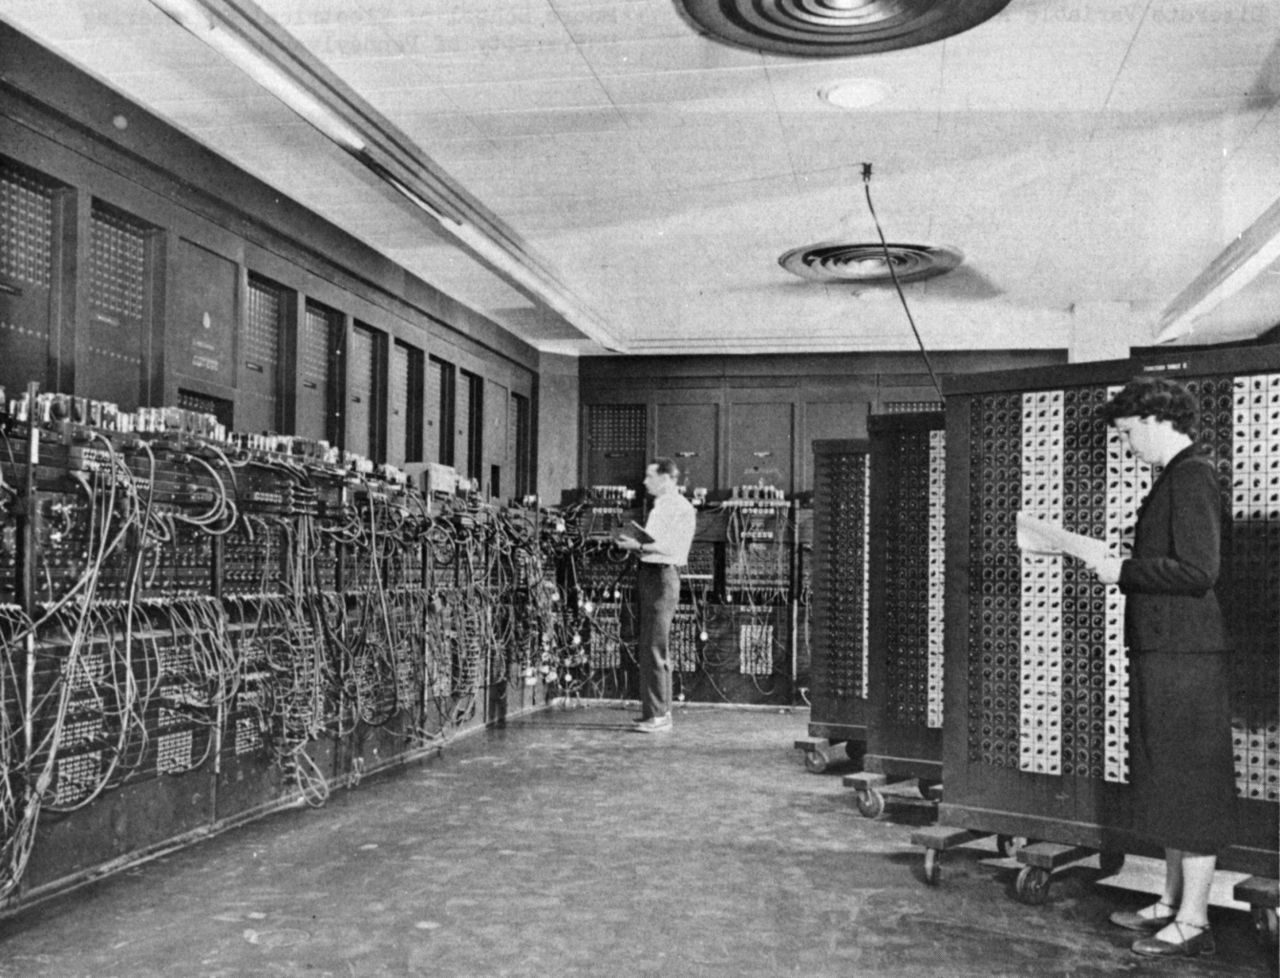
\includegraphics[height=0.75\textheight]{./img/eniac.jpg}
\end{frame}

%%%%%%%%%%%%%%%%%%%%%%%%%%%%%%%%%%%%%%%%%%%%%%%%%%%%%%%%%%%%%%%%%%%%%%%%%%%%%%%%
\begin{frame}[fragile]
  \frametitle{Algorithms}
\end{frame}

%%%%%%%%%%%%%%%%%%%%%%%%%%%%%%%%%%%%%%%%%%%%%%%%%%%%%%%%%%%%%%%%%%%%%%%%%%%%%%%%
\begin{frame}[fragile]
  \frametitle{Algorithms}

  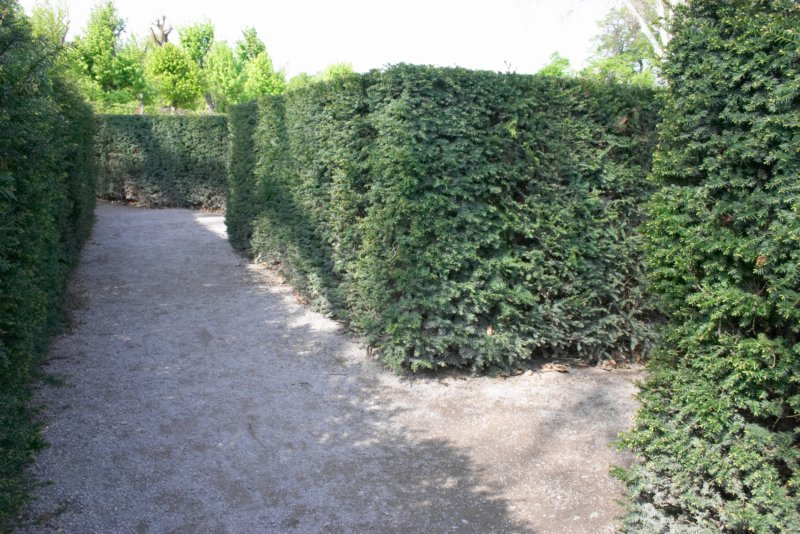
\includegraphics[height=0.75\textheight]{./img/hedge-maze.jpg}
\end{frame}

%%%%%%%%%%%%%%%%%%%%%%%%%%%%%%%%%%%%%%%%%%%%%%%%%%%%%%%%%%%%%%%%%%%%%%%%%%%%%%%%
\begin{frame}[fragile]
  \frametitle{Computing}

  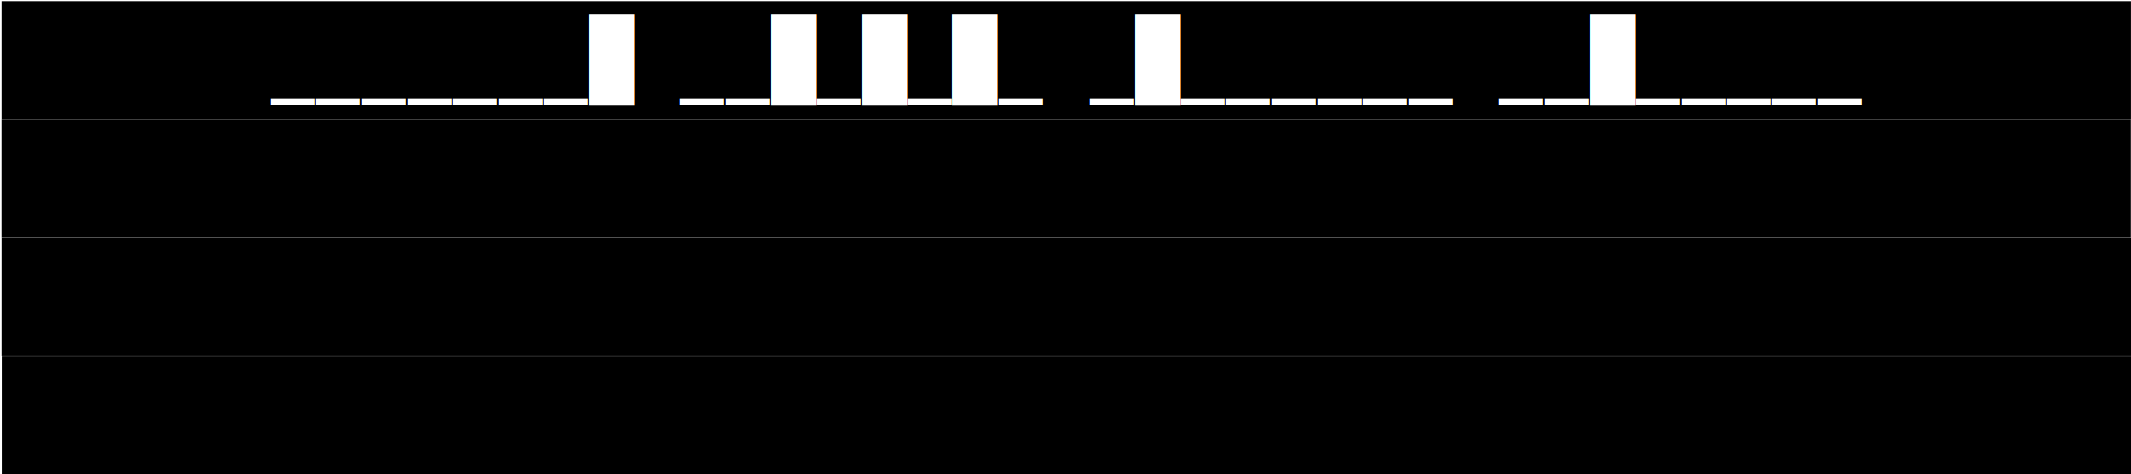
\includegraphics[width=\textwidth]{./img/assembler-1.png}
\end{frame}

%%%%%%%%%%%%%%%%%%%%%%%%%%%%%%%%%%%%%%%%%%%%%%%%%%%%%%%%%%%%%%%%%%%%%%%%%%%%%%%%
\begin{frame}[fragile]
  \frametitle{Computing}

  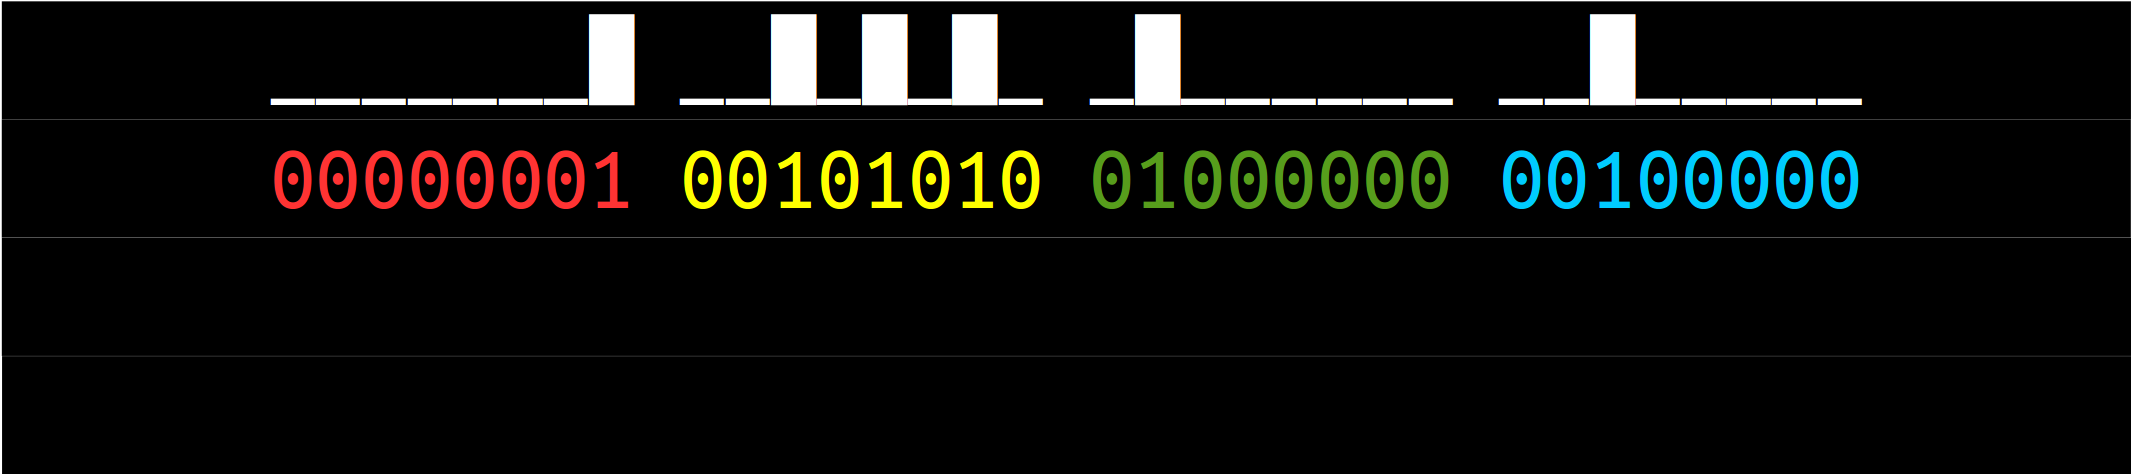
\includegraphics[width=\textwidth]{./img/assembler-2.png}
\end{frame}

%%%%%%%%%%%%%%%%%%%%%%%%%%%%%%%%%%%%%%%%%%%%%%%%%%%%%%%%%%%%%%%%%%%%%%%%%%%%%%%%
\begin{frame}[fragile]
  \frametitle{Computing}

  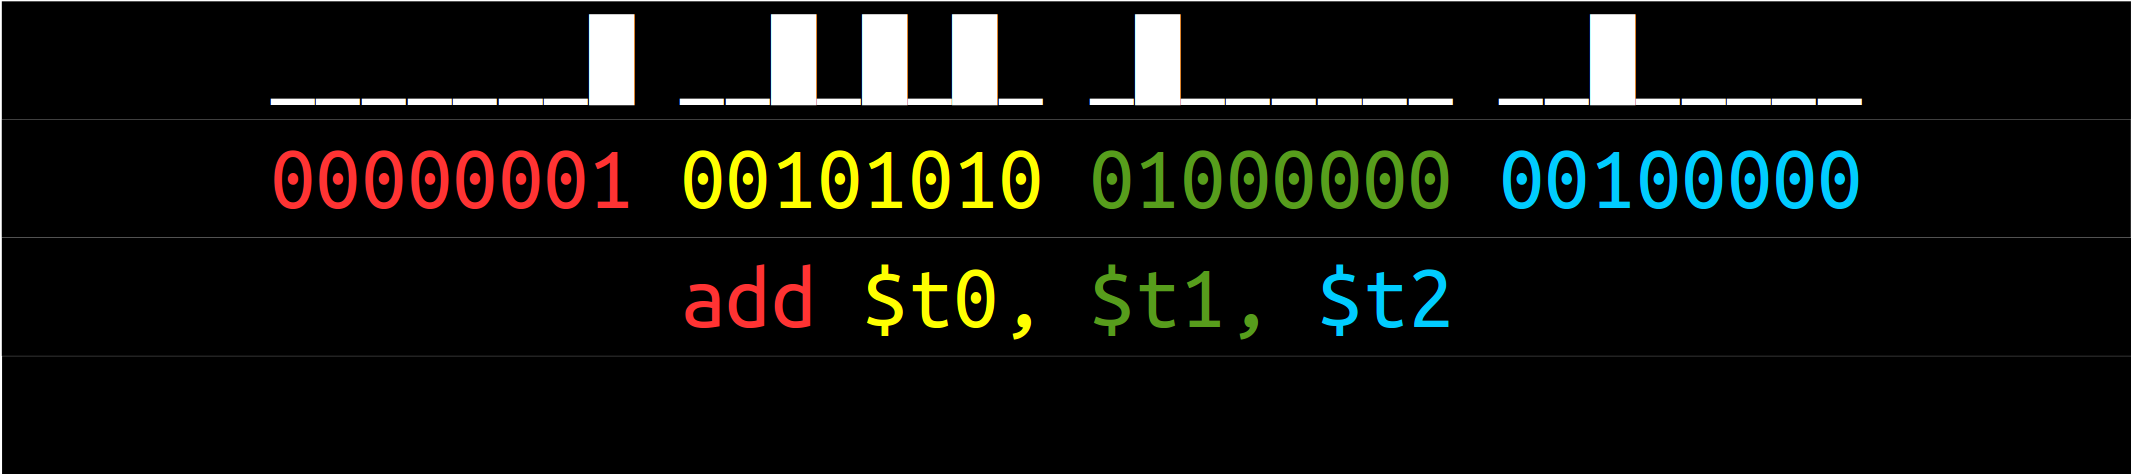
\includegraphics[width=\textwidth]{./img/assembler-3.png}
\end{frame}

%%%%%%%%%%%%%%%%%%%%%%%%%%%%%%%%%%%%%%%%%%%%%%%%%%%%%%%%%%%%%%%%%%%%%%%%%%%%%%%%
\begin{frame}[fragile]
  \frametitle{Computing}

  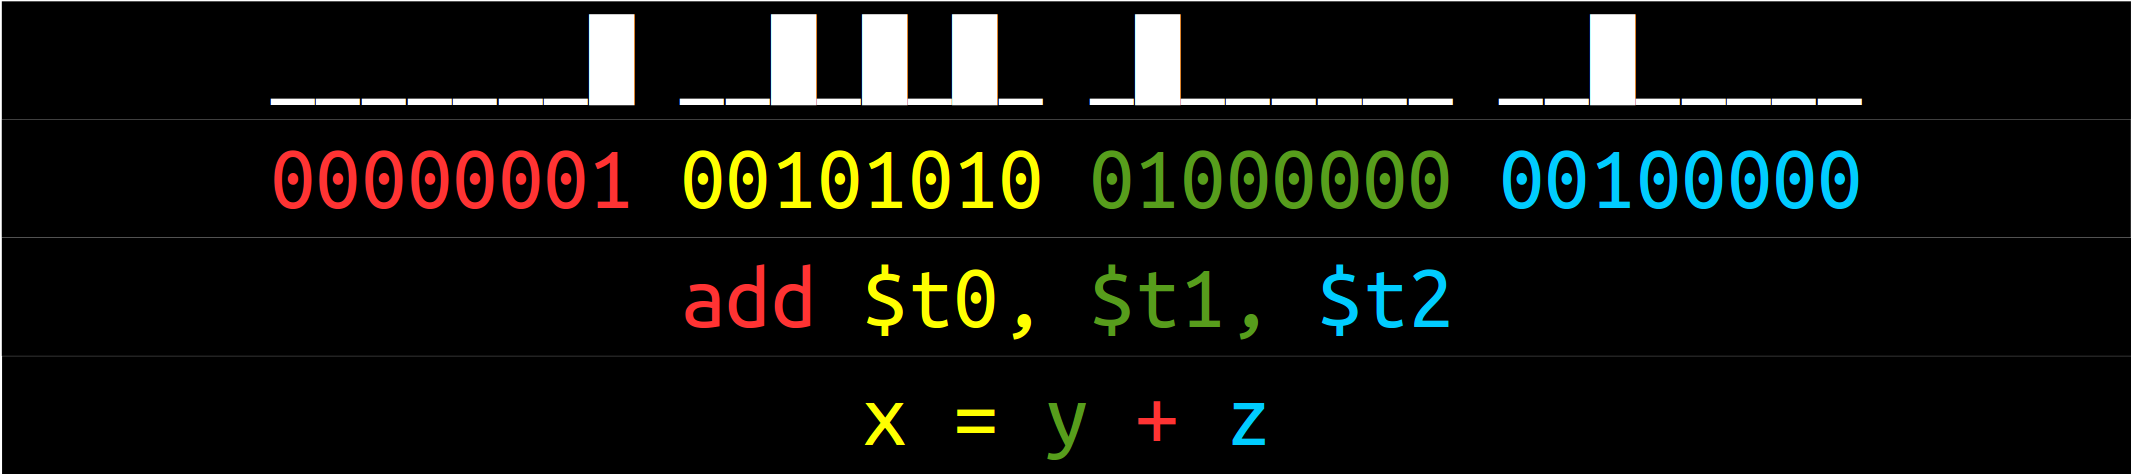
\includegraphics[width=\textwidth]{./img/assembler-4.png}
\end{frame}

%%%%%%%%%%%%%%%%%%%%%%%%%%%%%%%%%%%%%%%%%%%%%%%%%%%%%%%%%%%%%%%%%%%%%%%%%%%%%%%%
\begin{frame}[fragile]
  \frametitle{Algorithms}

  \begin{centering}
  
\includegraphics[width=0.5\textwidth]{./img/python-logo.png}
  \end{centering}
\end{frame}

%%%%%%%%%%%%%%%%%%%%%%%%%%%%%%%%%%%%%%%%%%%%%%%%%%%%%%%%%%%%%%%%%%%%%%%%%%%%%%%%
\begin{frame}[fragile]
  \frametitle{Algorithms}
  \Enlarge
%TODO
  \begin{Verbatim}[commandchars=\\\{\}]
\textcolor{CS101AltDark}{
depth * area = volume} \pause

\textcolor{CS101AltDark}{
volume of rain / volume per raindrop}
\textcolor{CS101AltDark}{
\hspace{2cm}= number of raindrops} \pause

\textcolor{CS101PureBase}{
volume_rain = area * depth} \pause

\textcolor{CS101PureBase}{
n_raindrops = volume_rain / volume_raindrop}
  \end{Verbatim}
\end{frame}

%%%%%%%%%%%%%%%%%%%%%%%%%%%%%%%%%%%%%%%%%%%%%%%%%%%%%%%%%%%%%%%%%%%%%%%%%%%%%%%%
\begin{frame}
  \frametitle{What is a program?}
  \Enlarge

  \begin{itemize} \pause
    \myitem A set of instructions a computer executes to achieve a goal.
  \end{itemize}
\end{frame}

%%%%%%%%%%%%%%%%%%%%%%%%%%%%%%%%%%%%%%%%%%%%%%%%%%%%%%%%%%%%%%%%%%%%%%%%%%%%%%%%
\begin{frame}
  \frametitle{What is data?}
  \Enlarge

  \begin{itemize} \pause
    \myitem Information stored in a computer. \pause
    \myitem All data is stored in binary.
  \end{itemize}
  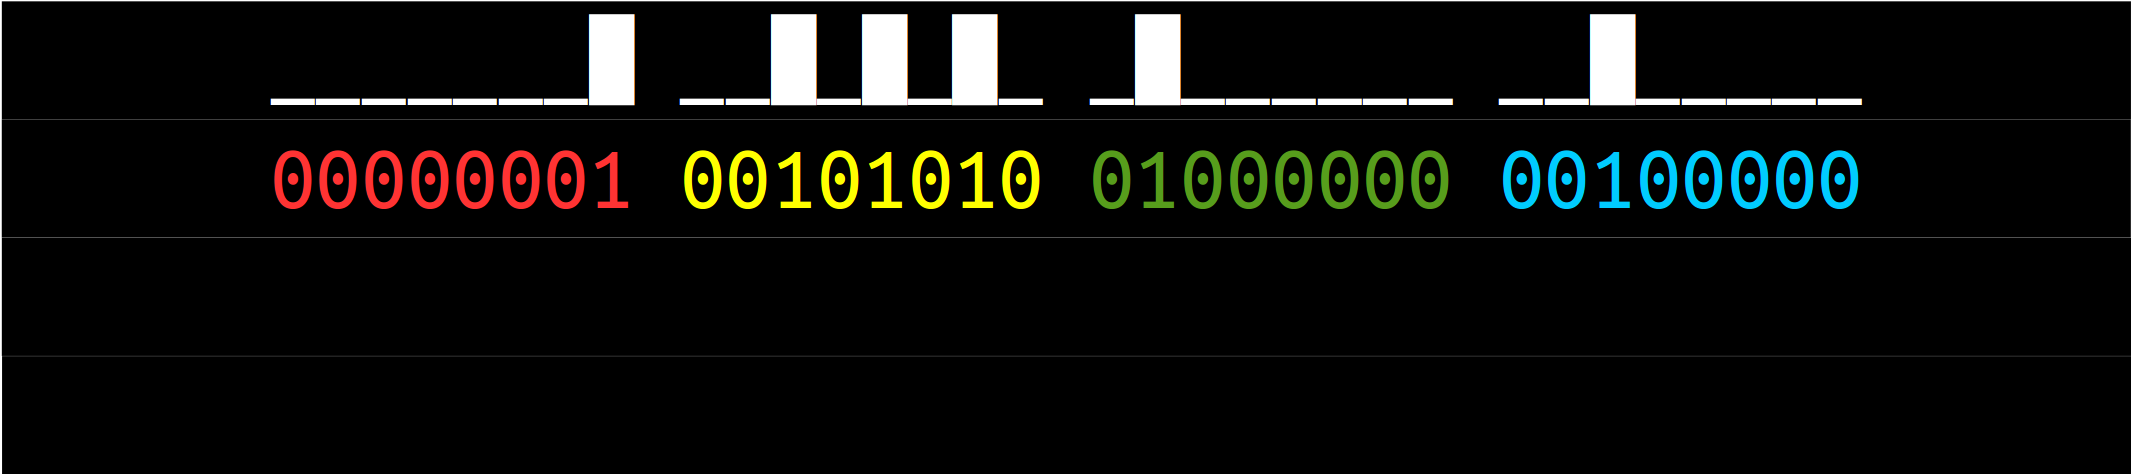
\includegraphics[width=\textwidth]{./img/assembler-2.png}
\end{frame}

%%%%%%%%%%%%%%%%%%%%%%%%%%%%%%%%%%%%%%%%%%%%%%%%%%%%%%%%%%%%%%%%%%%%%%%%%%%%%%%%
\begin{frame}
  \frametitle{What is data?}
  \Enlarge

  \begin{itemize}
    \myitem Binary data must be interpreted:
	\begin{itemize}
	  \mysubitem instruction \pause
	  \mysubitem value (number, character) \pause
	  \mysubitem memory location \pause
	\end{itemize}
  \end{itemize}
  \begin{centering}
  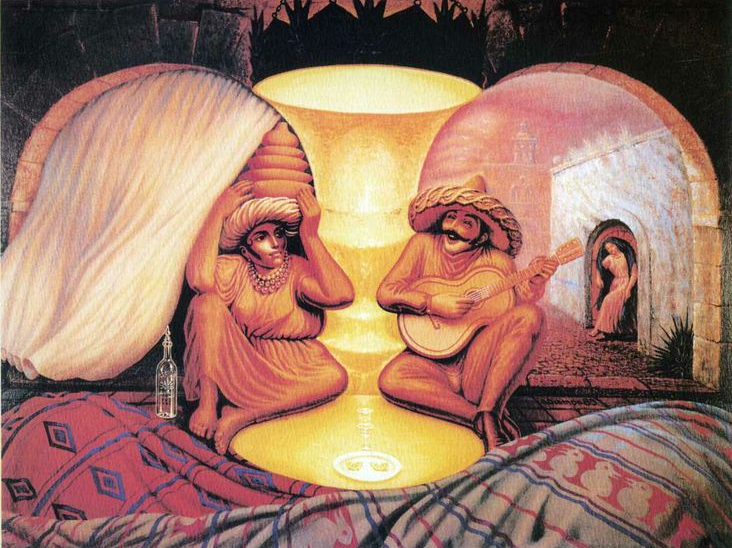
\includegraphics[height=0.5\textheight]{./img/dali.png}
  \end{centering}
\end{frame}

%%%%%%%%%%%%%%%%%%%%%%%%%%%%%%%%%%%%%%%%%%%%%%%%%%%%%%%%%%%%%%%%%%%%%%%%%%%%%%%%
\begin{frame}
  \frametitle{What is a program?}
  \Enlarge

  \begin{itemize} \pause
    \myitem Programs are data! \pause
	\myitem Instructions are encoded in binary.
  \end{itemize}
  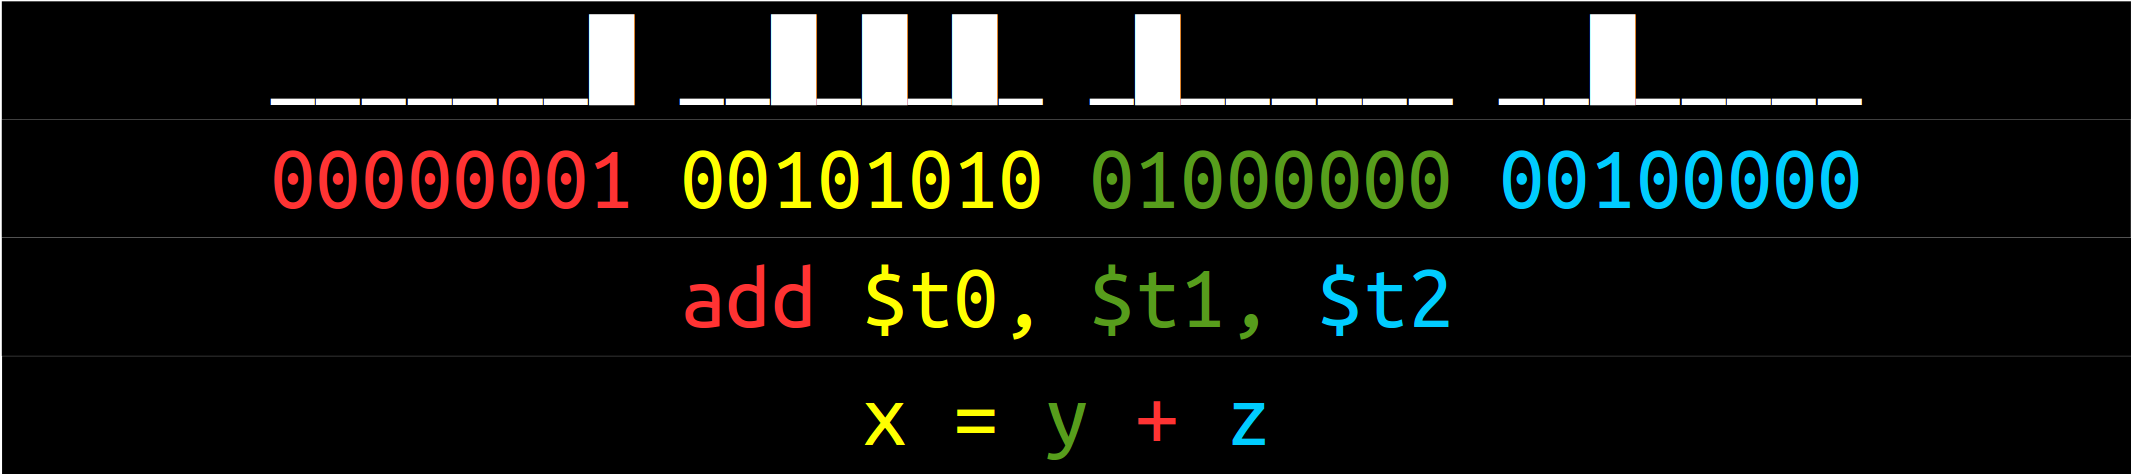
\includegraphics[width=\textwidth]{./img/assembler-4.png}
\end{frame}

%%%%%%%%%%%%%%%%%%%%%%%%%%%%%%%%%%%%%%%%%%%%%%%%%%%%%%%%%%%%%%%%%%%%%%%%%%%%%%%%
\section{Reminders}

%%%%%%%%%%%%%%%%%%%%%%%%%%%%%%%%%%%%%%%%%%%%%%%%%%%%%%%%%%%%%%%%%%%%%%%%%%%%%%%%
\begin{frame}
  \frametitle{Reminders}
  \Enlarge

  \begin{itemize}
  \myitem i>clicker \\ \textcolor{CS101GradBot}{\footnotesize\hspace{1em} Grades count starting Wed 08-31}
  \end{itemize}
  \begin{center}
    \textcolor{CS101Base}{\Huge \texttt{go.illinois.edu/cs101}}
  \end{center}
\end{frame}

\end{document}
